\chapter{Anforderungsanalyse}\label{chapter:anforderungsanalyse}
In diesem Kapitel werden die Anforderungen an die Anwendung und den zu entwickelnden Prototypen erhoben. Dazu wird zunächst auf Grundlage der Literatur ein Anwendungsfall erstellt und für diesen dann eine Anforderungsanalyse durchgeführt.


\section{Vision}
Die Anwendung hat den Bildungsbereich und das Lernen mit Hilfe von Augmented Reality als Zielgruppe. In der Arbeit von \citeauthor{diegmann:benefits-ar} werden dazu verschiedene Anwendungsarten definiert (vergleiche \ref{sec:diegmann-benefits-ar}). Diese stellt zudem auch das entdeckungsbasierte Lernen als die Einsatzmöglichkeit mit den meisten Vorteilen für das AR-gestützte Lernen heraus. In diese Kategorie fällt auch die in Abschnitt \ref{sec:atlas-humananatomie} vorgestellte Anwendung \glqq Atlas der Humananatomie 2020\grqq. \\
Die Anwendungen soll in der Art der Wissensvermittlung auf den selben, bereits im praktischen Einsatz getesteten Grundlagen beruhen. Sie soll Lernende unterstützen, indem sie ihnen dreidimensionale Modelle anzeigt. \\
Jedoch soll das Konzept von Anwendungen, wie \glqq Atlas der Humananatomie 2020\grqq dabei wie folgt erweitert werden:\\
Zum einem soll die Anwendung so aufgebaut werden, dass sie vom Nutzer speziell an die eigenen Bedürfnisse angepasst werden kann. Dazu soll die Anwendung kein festes Set an Modellen zur Verfügung stellen, sondern die Modelle können vom Nutzer hochgeladen werden. \\
Der zweite Punkt ist, dass anstelle des meistens verwendeten Matural Feature Tracking ein Markerbasiertes Tracking verwendet werden soll. So das die Modelle speziellen Dokumenten, Textpassagen oder Lerninhalten mit Hilfe der Marker zugeordnet werden können. Diese Marker könnten dann schnell und einfach mit der Kamera getrackt werden.\\
Außerdem ist es die Vision, das dieses Markerbasierte Tracking in einem großen Kontext genutzt werden kann. \\
Dazu wäre eine Umsetzung angelehnt an die Webseite Socrative.com denkbar. Diese Webseite bietet Professoren die Möglichkeit Umfragen über einen Raumcode mit den Studierenden zu teilen. \\
Ein ähnliches System könnte auch zum Teilen der Modelle genutzt werden, sodass der Professor die Marker verknüpft mit den entsprechenden Modellen in eine Präsentation zusammen mit einem Raumcode einfügen kann und der Studierende dann, sobald er den Raumcode eingegeben hat, die Modelle in seinem Kamerabild sieht, wenn der entsprechende Marker getrackt wurde.\\
Ein solcher Einsatz von Augmented Reality bietet die Möglichkeit eindimensionale Vorlesungen oder Unterrichtseinheiten um eine interaktive Komponente zu erweitern und sollte viele der in der Literatur erwähnten positiven Auswirkungen, wie 
eine Verbesserung der  Motivation, der Aufmerksamkeit des Verständnisses der Lerninhalte übertragen können (vergleiche Kapitel \ref{sec:diegmann-benefits-ar}). Auch Faktoren wie die von \citeauthor{billinghurst:ar-in-education} beschriebene Verbesserung der Kommunikation während der Interaktion mit digitalen Lernmethoden, wird unterstützt (vergleiche \ref{sec:billinghurst-ar-education}).

\section{Der Prototyp}
Im Rahmen der der Arbeit wurde dabei das folgende Konzept für einen vertikalen Prototypen entwickelt. \\
Dieser soll die Funktionalität des Verarbeitens eigener Modelle sowie das Tracken von selbst erstellten Markern testen.
Dazu soll der Fokus die Umsetzung der Augmented Reality und das Erstellen der zu trackenden Marker gelegt werden und die hoch geladenen Modelle sollen lediglich lokal gespeichert werden. \\
Dadurch handelt es sich bei dem Prototyp um die Umsetzung eines \glqq privaten Raumes\grqq . Er bietet dem Anwender nicht die Möglichkeit die Modelle zuteilen.\\ 
Eine ansonsten notwendige Datenspeicherung auf einem Server, das Implementieren eines Raumsystems mit Zugangscode und weitere Funktionen zum Teilen von Daten fallen dadurch weg.

\section{Anforderungsanalyse}\label{sec:Anforderungsanalyse}
Im folgenden wird eine Anforderungsanalyse für den zu entwickelnden Prototyp durchgeführt.
Dazu wurde das in der Softwaretechnik I Vorlesung vorgestellte Verfahren zur Anforderungsdefinition genutzt \citep[Folie 209-214]{winter:srs-anforderungen}. 
Dieses Verfahren sieht den folgenden Aufbau vor:
\begin{enumerate}
\item Vision 
\item Machbarkeitsstudie
\item Beschreibung der Systemumgebung
\item Anwendungsfälle
\item Anforderungsliste
\item Prototypen
\item Glossar
\end{enumerate}
Im folgenden wird jedoch nur eine vereinfachte, an diese Arbeit angepasste Version dieses Verfahrens genutzt.

\subsection{Beschreibung der Systemumgebung}
Bei dem Prototyp handelt es sich um eine mobile Anwendung. Das Endgerät für den Nutzer ist also ein Smartphone. \\
Der relevante Sensor, den das Smartphone für das Trackingverfahren bereitstellt, ist die Kamera. Die Anwendung muss die Videoframes analysieren und eine Ausgabe in Form von einem gerenderten 3D-Modell auf dem Display darstellen. \\

Insgesamt besitzt der Prototyp drei Unterfunktionen: \\
\begin{enumerate}
\item Das Generieren von Markern. Hierbei erstellt der Prototyp Marker für den Anwender, die alle eine unterschiedliche ID besitzen und aus jeder Rotation eindeutig zuerkennen sind. Dafür müssen sich zwei Marker auch unterscheiden, wenn einer von ihnen beliebig rotiert wurde.
\item Das Tracken von Markern. Bei dem die Anwendung einen Marker in einem Videoframe erkennt und seine Position und Transformation im Videoframe berechnet. Dabei liegt der Marker in gedruckter Form auf einem Blatt Papier vor oder wird auf einem Bildschirm angezeigt.
\item Das Rendern von Modellen. Das anzuzeigende Modell wurde dabei vom Nutzer  als Datei hochgeladen und muss zunächst vom System verarbeitet werden. Um im Anschluss das Modell realistisch in Relation zum Marker zu platzieren, muss die beim Tracking berechnete Position und Transformation des Markers verwendet werden. 
\end{enumerate}
Da der Prototyp auf einem mobilen Endgerät genutzt wird, variiert die Umgebung in welcher dieser zum Einsatz kommt stark. Deshalb ist es notwendig, dass das System robust gegenüber verschiedenen Umwelteinflüssen ist.\\


\subsection{Anwendungsfälle des Prototyps}
Ein Anwendungsszenario des Prototypen ist die mit dem Prototyp generierten Marker auf einem auf einem begleitenden Unterrichtsdokument einzufügen und ein oder mehrere relevante Modelle zu verlinken. Dazu werden die Modelle in dem Prototyp hochgeladen und lokal auf dem Gerät gespeichert. Die von der Anwendung generierten Marker können dann in einem Dokument eingefügt werden. Über die Kamerafunktion ist es im Anschluss möglich die Marker zu scannen, um sich die entsprechenden, dreidimensionale Modell anzeigen zu lassen.\\ 
Allgemein lassen sich die Funktionen und Anwendungsfälle in dem in Abbildung \ref{fig:Use-Cases} gezeigtem Anwendungsfalldiagramm visualisieren.
\begin{figure}[h!]
\centering
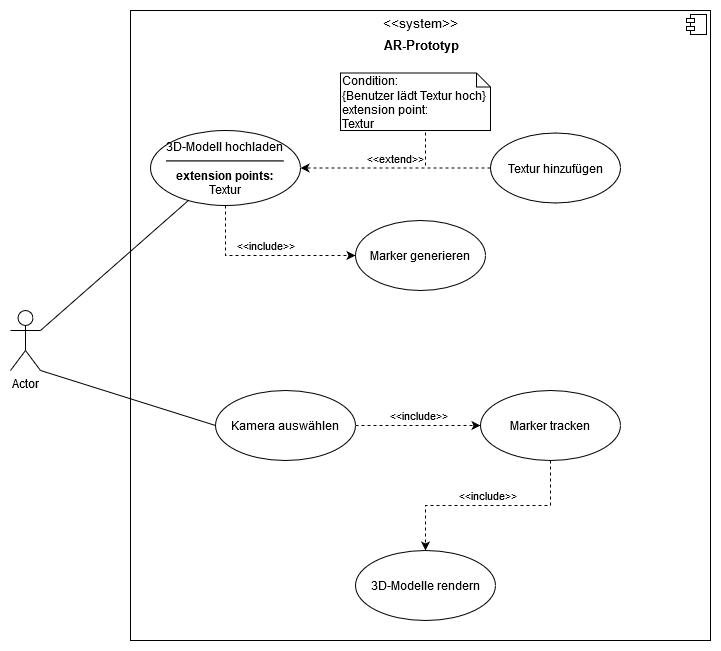
\includegraphics[width=1.0\textwidth]{Abbildungen/use-case-diagram.png}
\caption[Use Cases des Prototyps]{Use Case Diagramm des Prototyps. (Quelle: Eigene Darstellung)}
\label{fig:Use-Cases}
\end{figure}


\subsection{Anforderungsliste}
Im folgenden Abschnitt werden die Anforderungen an den Prototyp definiert. Dabei wird zwischen funktionalen und nicht-funktionalen Anforderungen unterschieden. 
\begin{quote}
\glqq Eine funktionale Anforderung ist eine Anforderung bezüglich des Ergebnisses eines Verhaltens, das von einer Funktion des Systems [...] bereitgestellt werden soll.\grqq \citep[S. 17]{rupp:requirements}
\end{quote}
Nicht-funktionale Anforderungen umfassen im Vergleich dazu die Anforderungen an die Technologie, die Qualität, die Benutzeroberfläche, die durchzuführende Tätigkeiten und rechtlich vertragliche Anforderungen \citep{rupp:requirements}.\\
Sie können als Eigenschaften, die das System besitzen muss, um den Nutzer zufrieden zustellen, beschrieben werden. \citep[S. 10]{robertson:requirements-process}. Diese Eigenschaften beziehen sich meistens auf die Bereiche Service Level, Zugriffsbeschränkungen, Sicherheit, Monitoring, Kontrolle, Schnittstellen, Archivierung, Benutzerfreundlichkeit und Konversion \citep[S. 139]{boehm:systementwicklung}. \\
Auf Grundlage dieser Definition wurden die folgenden funktionalen und nicht-funktionalen Anforderungen mit Hilfe der von \citeauthor[S. 219]{rupp:requirements} definierten Anforderungsschablonen aufgestellt:

\subsubsection{Funktionale Anforderungen}
\begin{itemize}
\item[FA01] Die Anwendung muss fähig sein, ein Marker zu generieren.
\item[FA02] Die Anwendung muss fähig sein, Marker in dem Kamerabild erkennen zu können.
\item[FA03] Die Anwendung muss fähig sein, generierte Marker zu unterscheiden.
\item[FA04] Die Anwendung muss dem Benutzer die Möglichkeit bieten, 3D-Modelle in Form von OBJ-Dateien hochzuladen können.
\item[FA05] Die Anwendung muss dem Benutzer die Möglichkeit bieten, Textur-Dateien im Bildformat(jpeg, png) hochzuladen.
\item[FA06] Die Anwendung muss fähig sein, hochgeladenen Dateien lokal zu speichern.
\item[FA07] Die Anwendung muss fähig sein, jedem Modell einen individuellen Marker zuzuordnen.
\item[FA08] Die Anwendung muss fähig sein, die dreidimensionalen Modelle im Kamerabild anzuzeigen.
\item[FA09] Die Anwendung muss fähig sein, die Transformation der Marker zu berechnen.
\item[FA10] Die Anwendung muss fähig sein, die Modelle basierend auf der berechneten Transformation zu rendern.
\end{itemize}

\subsubsection{Nichtfunktionale Anforderungen}
\begin{itemize}
\item[NF01] Das Endgerät der Anwendung sollte ein Android Smartphone(Huawei P30 Pro) sein.
\begin{enumerate}
\item[NF01.1] Die genutzte Entwicklungsumgebung der Anwendung sollte Android Studio sein.
\item[NF01.2] Die genutzte Programmiersprache der Anwendung sollte Java sein.
\end{enumerate}
\item[NF02] Die Markergenerierung der Anwendung sollte so gestaltet sein, dass es mindestens 10 verschiedene Marker generieren kann.
\item[NF03] Das Tracking der Anwendung sollte kamerabasiert sein.
\item[NF04] Das Tracking der Anwendung sollte auf einem markerbasiertem Verfahren beruhen.
\item[NF05] Das Tracking der Anwendung sollte mit mindestens 30FPS laufen.
\item[NF06] Das Tracking der Anwendung sollte so gestaltet sein, dass es alle generierten Marker der Anwendung erkennen kann.
\item[NF07] Bei vollständig erkanntem Marker sollte das Tracking robust gegenüber Rotation, Skalierung, Perspektive und Belichtung sein.

\item[NF08] Die Benutzeroberfläche der Anwendung sollte eine einfache Navigation zu allen Komponenten der Anwendung bereitstellen.
\item[NF09] Die Benutzeroberfläche der Anwendung sollte eine Ansicht zum Hochladen und Verwalten der Modelle bieten.
\item[NF10] Die Benutzeroberfläche der Anwendung sollte einen Zugriff auf die Kamera ermöglichen.








\end{itemize}

